\begin{figure*}[hbt]
\centering
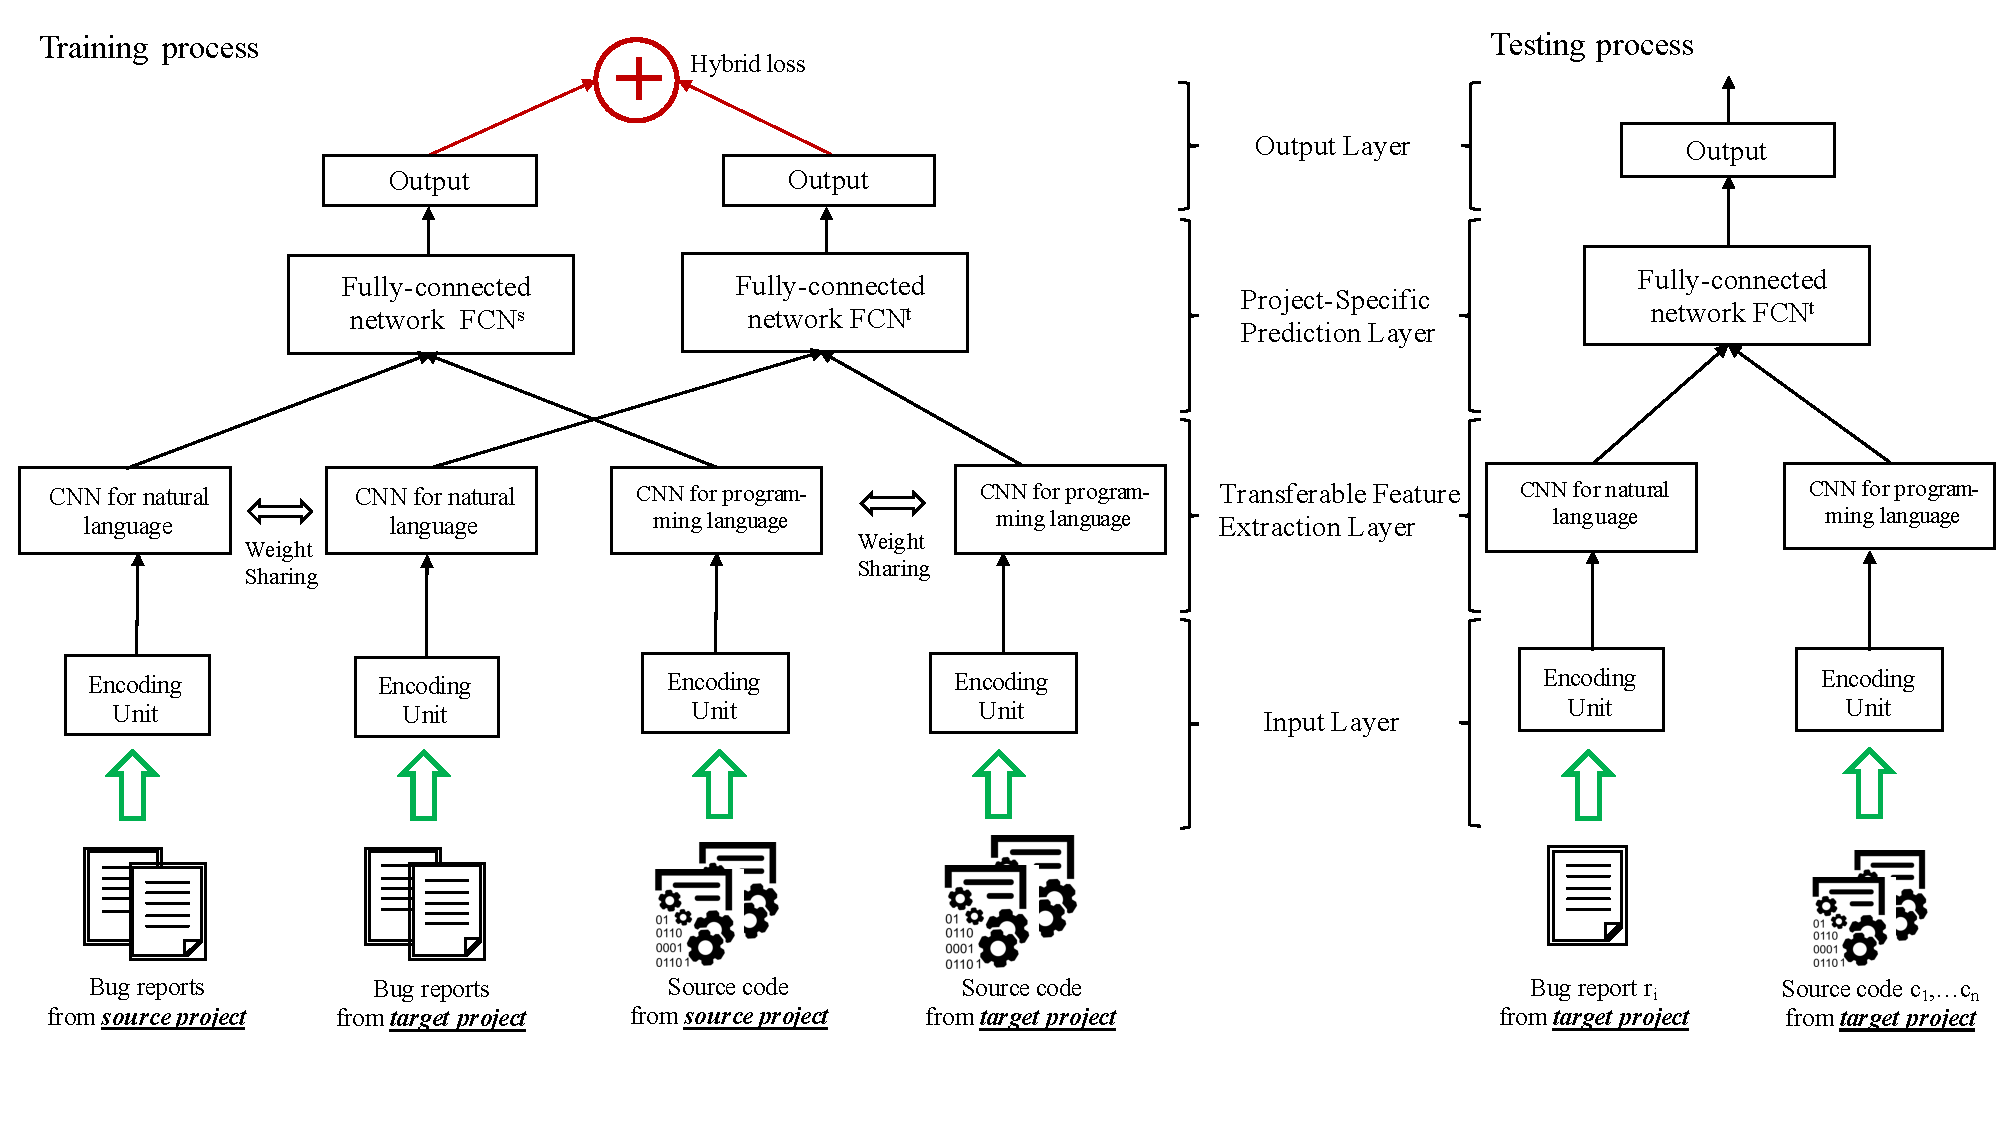
\includegraphics[width = 2\columnwidth]{pic/structure.pdf}
\caption{The overall structure of Transfer Natural and Programming language CNN.  The left part is the training process of \TRANPCNN based on the bug reports and source code from source projects and a few data from target projects, the weights of which are trained by minimizing the loss of ensemble loss from fully-connected networks $fc_s$ and $fc_t$. The right part is the testing process, a new bug report and its candidate source code are fed into the model, and \TRANPCNN outputs their relevant scores for bug localization.}
\label{fig:structure}
\end{figure*}


The goal of cross-project bug localization is using data from source project and a few data from target project to locate the potentially buggy source code in the target project that produce the program behaviors specified in a given bug report.  Let $\mathcal{C}^s =   \{ { c^s_1, c^s_2}, \cdots, c^s_{n^c_1} \} $ and $\mathcal{C}^t =\{ c^t_1, c^t_2, \cdots, c^t_{n^c_2} \}$ denote the set of source code from source project and target project respectively, $\mathcal{C}=\mathcal{C}^s \bigcup \mathcal{C}^t $. 
$\mathcal{R}^s =\{ r^s_1, r^s_2, \cdots, r^s_{n^r_1} \}$ and $\mathcal{R}_t =\{ r^t_1, r^t_2, \cdots, r^t_{n^r_1} \}$ denotes the bug reports, respectively, $\mathcal{R}=\mathcal{R}^s \bigcup \mathcal{R}^t $, where $n^c_1, n^c_2, n^r_1, n^r_2$ denote the number of source files and bug reports from source project and target project, respectively. We formulate cross-project bug localization as a learning task which firstly learn a prediction function $f: \mathcal{R}^s \times \mathcal{C}^s \mapsto \mathcal{Y}^s$. $y^s_{ij} \in \mathcal{Y}^s = \{ +1, -1 \}$ indicates whether a source code $c^s_j \in \mathcal{C} $ is relevant to a bug report $r^t_i \in \mathcal{R}$ in the source project, and then learn the prediction function $f: \mathcal{R}^t \times \mathcal{C}^t \mapsto \mathcal{Y}^t$, indicates the labels of pairs of source code and bug reports in target domain. 

In this paper, we propose a novel deep transfer neural network named \TRANPCNN (TRAnsfer Natural and Programm Language Convolutional Neural Network) to instantiate the cross-project bug localization problem. \TRANPCNN takes the raw data of bug reports and source code from different projects as inputs and learns a prediction function to predict the related labels or a given bug report $r^t_i$ and source code $c^t_j$ from target projects. The key point of \TRANPCNN is that the feature representation process is similar among cross projects, which is transferable and can be trained using the data from both source and target project so that the source project is able to help train a more functional feature extraction model. Then \TRANPCNN employs two models for prediction from source project and target project, respectively, to avoid the influence of inconsistency data distribution. We will introduce the general framework of \TRANPCNN and explain the way to employ deep transfer technique for cross-project bug localization in the following subsections.

\subsection{Model Structure}
The model structure of \TRANPCNN is depicted in Figure~\ref{fig:structure}, where the subfigure to the left depicts the training process of \TRANPCNN, while subfigure to the right depicts the corresponding test process. 

\TRANPCNN consists four parts: the input layer, the transferable feature extraction layers, project-specific correlation fitting layers and the output layer. The input layer takes the bug report as well as the source code in its original format and generate their corresponding encodings such that they can be further processed by the subsequent layers of \TRANPCNN; the transferable feature extraction layers aim to learn the intermediate feature representations from the bug reports and source codes, respectively, such that the common knowledge shared by both the source project and the target project which can eventually facilitate the identification of the correlation between the bug report and the source codes; the project-specific prediction layer is responsible for biasing the learning based on the transferable feature representation towards the project-specific correlation patterns between the bug reports and source codes in source project and target project, respectively; the output layers generate the final correlation scores for the report-code pairs based on the fitted correlations in the source domain and the target domain, respectively. It is obvious that the the transferable feature extraction layers and project-specific correlation fitting layers are the key parts of the proposed model, which would be explained in details in the following subsections.

To train this model, report-code pairs from the source project and target project along with their ground truth correlation labels are fed into the proposed deep model in order to learn the transferable feature representation shared by both source and target projects as well as the project-specific prediction functions for the source and target project, respectively. After the model is fully trained, prediction function $f^{t}$ would be used for determine the correlation of the report-code pair $(r_i^t, c_j^t)$ from the target project.

\subsection{Transferable Feature Extraction Layer}
When provided with the bug report and codes from the source and target project in their original format, the encodings for the bug reports and the source codes are first generated by the preceded input layer. Traditional TFIDF representation fails to capture correlation between terms. Thus, we employ word2vec encoding to represent both the bug reports and the source codes in the purpose of enriching the initial representation, based on which, the transferable features are further extracted.

The transferable features for bug report and the source codes should satisfy the following properties. First, the transferable features should be able to represent the functional semantics in both bug reports and source codes such that the semantics can be further utilized to identify the correlation patterns between the reports and the codes. Second, the extract semantics should be able to embed some common knowledge between the source project and target project such that those knowledge learned from the source project can be eventually transferred to facilitate the learning for the target project.

To make the embedded knowledge to be transferable between source and target projects, the key challenge here is how to identify what information is useful and transferable and what is useful but may not be transferred to other projects. To address this challenge, we employ a special strategy called \emph{weight sharing} during the learning process, which imposes a hard constraint that the learned weights in the network (either N-CNN or P-CNN) for the target project should be exactly the same as the the learned weights in the network for the source project. By weight sharing, the learning procedure that facilitates good performance on both source project and target project is forced to focus on those common features shared by both source project and target project rather than extracting the project-specific features for each project. Thus, the resulting features eventually \emph{transfer} the common knowledge that are useful for determine the correlation between the bug report and the source code from the source project to the target project. Note that such knowledge may need a large amount of labeled training data to be learned for any single project, but now can be directly used for the target project where the labeled training data may be limited especially for the code start. 

\subsection{Heterogeneous Predicting Adaptation Layers}
After processing from transferable feature extraction layers, the high-level semantic features from bug reports and source code are extracted, which would be then fed into a fully-connected neural network for feature fusion. However, in cross-project bug localization, the data distribution of source project and target project is different, which means directly employing the same fully-connected network to fuse features from both source and target projects will have bias, leading to a poor bug localization performance.

One question arises here: can we design a particular network to extract features within project, and fuse feature in separate structure? To address this problem, we design two particular fully-connected networks to combine the middle-level features in Cross-project feature fusion layers: One fully-connected network $fc_s$ is used for source project feature fusion and the other fully-connected work $fc_t$ is used to fuse features in the target project. The structure suggests that the feature extraction of different projects are similar and can be processed in the same Convolutional Neural Network, and the feature fusion and projection process is different so that two separate fully-connected neural network are designed to solve this problem. The objective function in the cross-project feature fusion layers can be rewritten in Eq.~(\ref{eq:lossfunction}):
\begin{equation}
\begin{aligned}
\label{eq:lossfunction}
\mathop{\arg\min}_{\mathbf{W}}&\sum_{s_i,s_j}\mathcal{L}(\mathbf{h}_{s_i},\mathbf{h}_{s_j}
,y_{s_{ij}}; W_{fc_s}, W_{conv} ))\\
+&\sum_{t_i,t_j}\mathcal{L}(\mathbf{h}_{t_i},\mathbf{h}_{t_j},y_{t_{ij}}; W_{fc_t}, W_{conv})+\lambda||\mathbf{W}||^2
\end{aligned}
\end{equation}
where, $\mathcal{L}$ is the square loss, $\lambda$ is the trade-off parameter and the weight vectors $W$ contains the weight vectors in convolutional neural networks $W_{conv}$, in fully-connected network of source domain $W_{fc_s}$ and in fully-connected network of target domain $W_{fc_t}$. All the weights is learned by minimizing the objective function based on SGD (stochastic gradient descent) in the same time.


%cross-language feature fusion layers, where a fully-connected network is employed for learning a unified features and followed by an output layer mapping to the predictions $\mathcal{Y}$. However, a reported bug may only relevant to one or a few source code, while a large number of source code are irrelevant and this imbalance nature should be considered. Similar to~\cite{huo2016learning} which introduced an unequal misclassification cost to handle imbalance problem, we randomly drop some negative instances in the cross-language feature fusion layer, which can decrease the computational cost and counteract the negative influence of the imbalance nature. Let $y_{i}^{(k)}$ denote the $k$-th label of instance $\mathbf{x}_i$ and $\tilde{y}_{i}^{(k)}$ denote its prediction, similar to traditional LSTM model, we use cross entropy error function in the output layer, and the parameters are learned by minimizing the following loss function using stochastic gradient descent (SGD) method: 